\documentclass[final]{beamer}
\usepackage{gensymb}
\usepackage{textcomp}
\usepackage[scale=1.24]{beamerposter} 

\definecolor{darkbg}{HTML}{171D1C}
\definecolor{lighttext}{HTML}{FFFFFF}
\definecolor{darktext}{HTML}{171D1C}
\definecolor{accent}{HTML}{DB9D47}
\definecolor{accent2}{HTML}{8CC084}

\usetheme{confposter} % Use the confposter theme supplied with this template
\setbeamercolor{block title}{fg=darkbg,bg=accent!80} % Colors of the block titles
\setbeamercolor{block body}{fg=darktext,bg=accent!10} % Colors of the body of blocks
\setbeamercolor{block alerted title}{fg=lighttext,bg=darkbg} % Colors of the highlighted block titles
\setbeamercolor{block alerted body}{fg=darktext,bg=accent!80} % Colors of the body of highlighted blocks

% Many more colors are available for use in beamerthemeconfposter.sty
%----------------------------------------------------------------
% Define the column widths and overall poster size
% To set effective sepwid, onecolwid and twocolwid values, first choose how many columns you want and how much separation you want between columns
% In this template, the separation width chosen is 0.024 of the paper width and a 4-column layout
% onecolwid should therefore be (1-(# of columns+1)*sepwid)/# of columns e.g. (1-(4+1)*0.024)/4 = 0.22
% Set twocolwid to be (2*onecolwid)+sepwid = 0.464
% Set threecolwid to be (3*onecolwid)+2*sepwid = 0.708
\newlength{\sepwid}
\newlength{\onecolwid}
\newlength{\twocolwid}
\newlength{\threecolwid}
\setlength{\paperwidth}{48in} % A0 width: 46.8in
\setlength{\paperheight}{38.4in} % A0 height: 33.1in
\setlength{\sepwid}{0.024\paperwidth} % Separation width (white space) between columns
\setlength{\onecolwid}{0.21\paperwidth} % Width of one column
\setlength{\twocolwid}{0.464\paperwidth} % Width of two columns
\setlength{\threecolwid}{0.708\paperwidth} % Width of three columns
\setlength{\topmargin}{-0.75in} % Reduce the top margin size

%----------------------------------------------------------------
\usepackage{graphicx}  % Required for including images
\usepackage{booktabs} % Top and bottom rules for tables
%----------------------------------------------------------------
\title{
False memories to fake news: The evolution of the term ``misinformation'' in academic literature
} 

\author{Alejandro Ruiz, Danny Benett, Julia Zimmerman, Christopher M. Danforth, Peter Sheridan Dodds}
\institute{Computational Story Lab, Vermont Complex System Center}
\addtobeamertemplate{headline}{} 
{
    \begin{tikzpicture}[remember picture,overlay] 
    \node [shift={(-10cm,-10cm)}] at (current page.north east) {
\includegraphics[height=6cm]{figures/uvm.jpg}}; 
    \end{tikzpicture}
    
    \begin{tikzpicture}[remember picture,overlay] 
    \node [shift={(-20cm,-10cm)}] at (current page.north east) {
\includegraphics[height=6cm]{figures/csc.png}}; 
    \end{tikzpicture}
    
    \begin{tikzpicture}[remember picture,overlay] 
    \node [shift={(-100cm,-10cm)}] at (current page.north east) {
\includegraphics[height=6cm]{figures/phd.png}}; 
    \end{tikzpicture}
    
    \begin{tikzpicture}[remember picture,overlay] 
    \node [shift={(-110cm,-10cm)}] at (current page.north east) {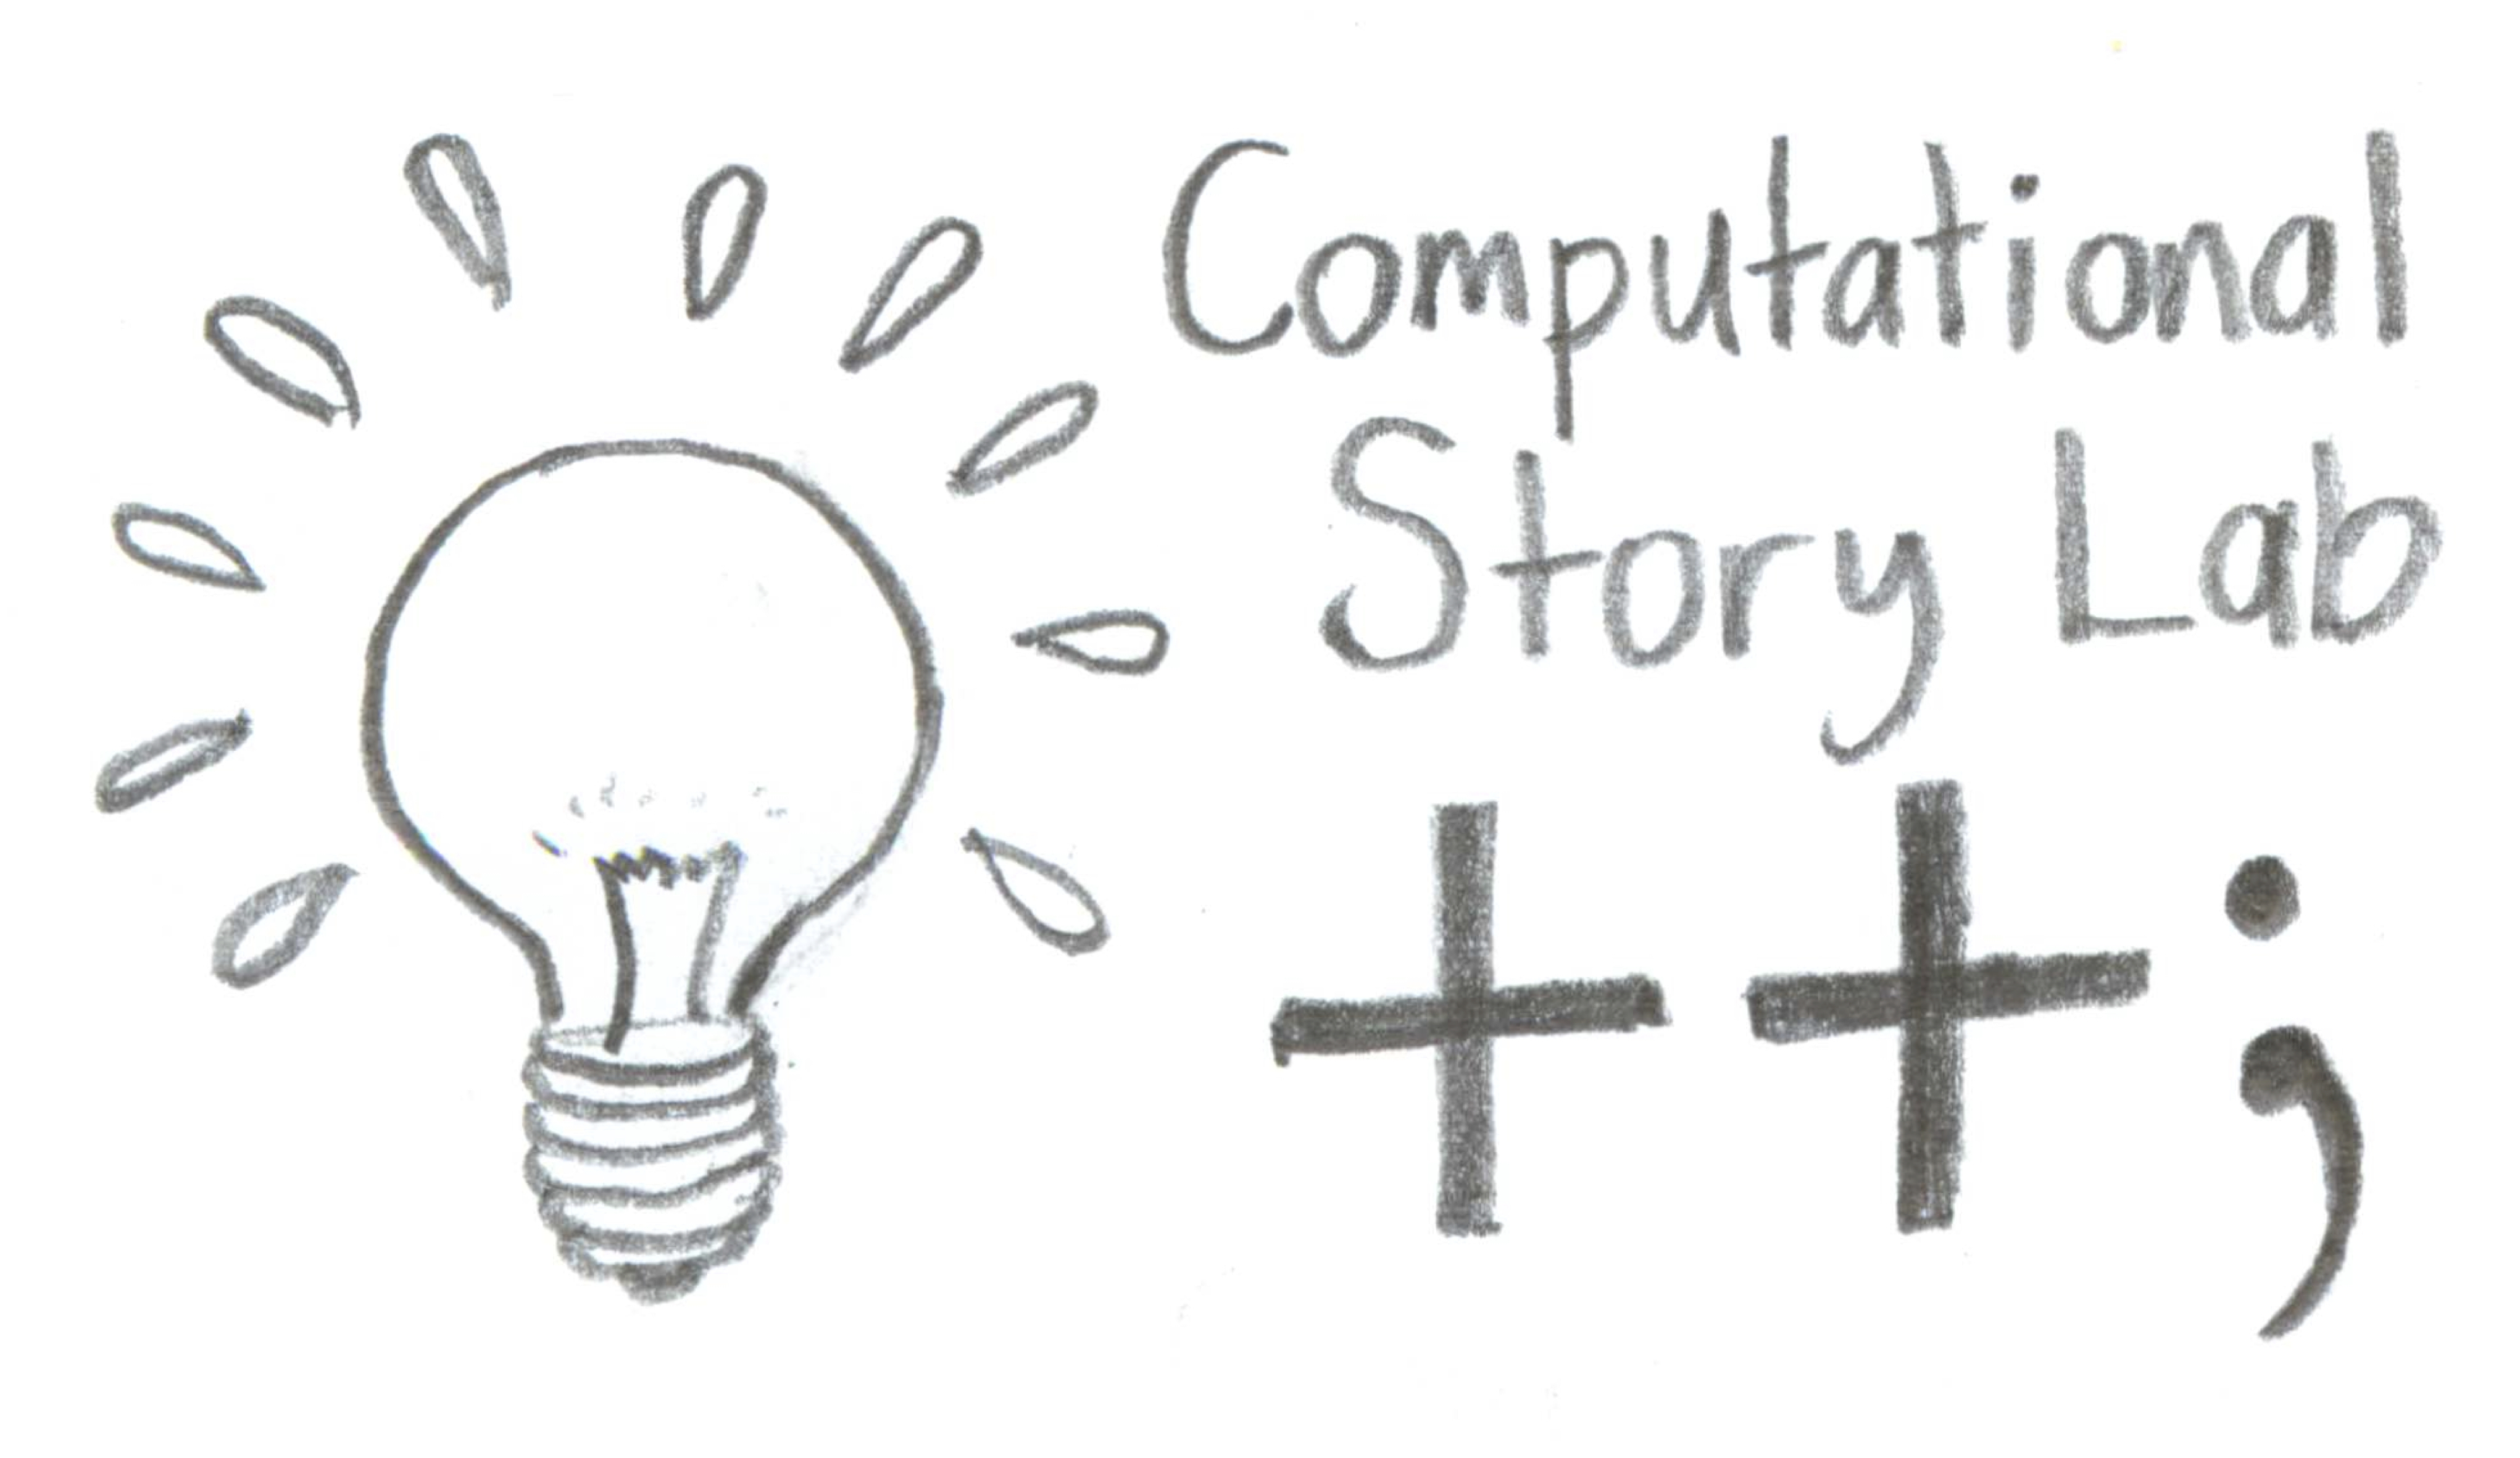
\includegraphics[height=6cm]{figures/storylab.jpg}}; 
    \end{tikzpicture}
}


\begin{document}

\begin{frame}[t] % The whole poster is enclosed in one beamer frame
\begin{columns}[t] % The whole poster consists of three major columns, the second of which is split into two columns twice - the [t] option aligns each column's content to the top
%----------------------------------------------------------------
  \begin{column}{\sepwid}\end{column} % Empty spacer column



\begin{column}{0.95\onecolwid} % The first column
\begin{block}{Twitter usage of ``misinformation''}
\begin{figure}

\includegraphics[width=1.0\linewidth]{misc-img/storywrangler.pdf}
\end{figure}
    
  \end{block}

\begin{block}{In academic literature}
\small    
  \begin{itemize}    
    \item 1956: "Combating Food Misinformation and Quackery"
    \item 1957: "Information and Misinformation Gained from Fasting Blood Sugar Alone in Diabetes Therapy"
    \item 1970: "A Model of the Soviet Firm" 
    \begin{itemize}
      \footnotesize
      \item Soviet firms’ attempts to correct for “systematic misinformation” by changing incentives
      \end{itemize}
    \item \textbf{1974: "Reconstruction of automobile destruction: An example of the interaction between language and memory"}
    \begin{itemize}
        \item Introduces the "misinformation effect" 
    \end{itemize}
    \item 1989: "Categorical Approach to Distributed Systems, Expressibility and Knowledge [...' the adversary should be chosen not to send identical faulty messages but to 'convey' the same misinformation"
    \item 2002: "Infodemiology: The Epidemiology of (Mis)Information"
    \begin{itemize}
      \item "The study of the determinants and distribution of health information and misinformation"
      \item 2007--2010 - Infodemiology extends to study how (mis)information spreads during crises (earthquakes, epidemics, etc.) on social media
    \end{itemize}
    \item 2016: The post-2016 paradigm is born
  \end{itemize}
\end{block}
\begin{block}{``Misinformation effect'' \\ and the Satanic panic}
\small
    \begin{itemize}
      \item The misinformation effect refers to the susceptibility of memories of an event to change when exposed to, for example, misleading questions
      \item The Satanic panic enters the mainstream with \textit{Michelle Remembers}, in which a recovered-memory patient and her doctor/soon-to-be-husband recount her (fabricated) childhood of torture by a Satanic cult
    \end{itemize}

\end{block}    
\end{column} % End of the first column

%----------------------------------------------------------------
\begin{column}{\sepwid}\end{column} % Empty spacer column
\begin{column}{1.05\twocolwid} % Begin a column which is two columns wide (column 2)

\large The \textbf{misinformation paradigm} studies people making, reading, and sharing \textbf{false statements}, usually on \textbf{social media}. It often produces research warning of the harm to society resulting from the sum of many such events.  

\begin{figure}

\includegraphics[width=1.0\linewidth]{term_frequency-img/fig.pdf}
\end{figure}
\begin{figure}
\includegraphics[width=1.0\linewidth]{network-img/both-communities.pdf}
\end{figure}

\end{column} % End of the second column

\begin{column}{\sepwid}\end{column} % Empty spacer column

\begin{column}{.95\onecolwid}
\begin{block}{Birth of the post-2016 paradigm}
  \begin{figure}
    
\includegraphics[width=1.0\linewidth]{network-img/1085.pdf}
  \end{figure}
\end{block}

\begin{block}{Theoretical Problems}
  \begin{itemize}
    \item \textbf{No theory of medium}: Misinformation paradigm sees through the medium, often discussing \textbf{direct} user interaction
    \item \textbf{Zombie laboratory model}: The core model from misinformation effect research is detached from its real world phenomenon
    \item \textbf{Lack of emergent theory}: Paradigm contains untenable theoretical commitment to evaluating individual pieces of information 
  \end{itemize}    
\end{block}

\begin{block}{Lack of emergent theory}
  \begin{itemize}
    \item  Researchers often define misinformation as social media posts that includes links to known unreliable sources
    \item  Public relations, military propaganda, intelligence agencies, etc. operate in the chasm between true and false, rather than at its poles
    \item  The more likely that a piece of misinformation is to be believed, the more difficult it necessarily is to detect as misinformation
    \item Untenable theoretical commitments force misinformation scholars to focus their inquiry precisely on the least salient part of the phenomenon
  \end{itemize}    
\end{block}

\end{column} 


% ----------------------------------------------------------------


\end{columns} % End of all the columns in the poster
\end{frame} % End of the enclosing frame
\end{document}
